\chapter{Evolutionary Limits} \label{ch:evolutionary limits}
This chapter inspects evolutionary limits predicted by Vose using infinite population model under no selective pressure. It states predicted orbits of infinite population and also discusses necessary and sufficient conditions are discussed. This section also explains implementation of simulation of evolutionary limits.

\section{Limits}
\label{Limits}
Vose states under mild assumptions on mutations (considered later), populations converge under repeated application of $\mathcal{M}$. Vose mentions that in general case, periodic orbits are possible but populations converge under repeated application of $\mathcal{M}^2$ and limits $p^\ast = lim_{n \rightarrow \infty} \mathcal{M}^{2n}(p)$ and $q^\ast = lim_{n \rightarrow \infty} \mathcal{M}^{2n+1}(q)$ exist.

Following Vose's theorem, let $S_g = g \mathcal{R} / \{\textbf{0}, g\}$, and let $|g|$ be the number of non zero bits in $g$.
\[
{{\widehat{p}}_g}^{\prime}  = \begin{cases}
    2^{\ell /2}  & \text{if $g = 0$}\\
    x_g \widehat{p}_g + y_g(\widehat{p}_g) & \text{otherwise}
  \end{cases}
\]
where,
\[
x_g = 2\widehat{M}_{g,0},  \hspace*{1cm} y_g(z) = 2^{\ell /2} \sum_{i \in S_g} z_i z_{i+g} \widehat{M}_{i,i+g}.
\]

Moreover, 
\begin{eqnarray*}
|g| & = & 1 \nudge \Rightarrow y_g = 0 \\
|g| & > & 0 \nudge \Rightarrow |x_g| \leq 1 \\
|x_g| & = & 1 \nudge \Rightarrow y_g = 0
\end{eqnarray*}

With above notations, limits can be expressed in Walsh basis by recursive equations 
\begin{equation}
\label{lt1}
\widehat{p^{\ast}}_g  = \begin{cases}
    (x_g y_g(\widehat{p^{\ast}}) + y_g(\widehat{q^{\ast}}))/(1-x_g^2)  & \text{if $|x_g| < 0$}\\
    \widehat{p}_g  & \text{otherwise}
  \end{cases}
\end{equation}
\begin{equation}
\label{lt2}
\widehat{q^{\ast}}_g  = \begin{cases}
    (x_g y_g(\widehat{q^{\ast}}) + y_g(\widehat{p^{\ast}}))/(1-x_g^2)  & \text{if $|x_g| < 0$}\\
    \widehat{\mathcal{M}(p)_g}  & \text{otherwise}
  \end{cases}
\end{equation}

If $x_g \neq −1$ for all $g$, then $p^\ast = q^\ast = lim_{n \rightarrow \infty} \mathcal{M}(p)$ is the limit of mixing. In other cases, 
mixing converges to a periodic orbit oscillating between $p^\ast$ and $q^\ast = \mathcal{M}(p^\ast)$.

Limits $\widehat{p^{\ast}}_g$ and $\widehat{q^{\ast}_g}$ can be computed considering $g$th components in order of increasing $|g|$ and 
performing complete indcution on $|g|$. If $|g| = 0$ then $g = 0$. Since $\widehat{p^\ast}_0 = 2^{-\ell/2}$ for all distributions $p$, 
the $\textbf{0}$the components of the sequence $\mathcal{M}^n(p)$ are identical in the Walsh basis. Since $|x_0| = 2$ ($x_g = 2\widehat{M}_{g,0}$ 
and $\widehat{M}_{0,0} = 1$), $\widehat{p^{\ast}}_g = \widehat{q^{\ast}}_g = 2^{-\ell/2}$. Next, consider $|g| = 1$. $y_g = 0$ for $|g| = 0$ 
(noted from above). These two cases $|g| < 2|$ are base cases for complete induction on $|g|$. The inductive hypothesis given by Vose is that 
for $|k| < |g|$, the $k$th component of $\mathcal{M}^n(p)$ in the Walsh basis converges to $\widehat{p^{\ast}}_k$ or $\widehat{q^{\ast}}_k$ as 
$n \rightarrow \infty$ through even or odd values respectively, and if $x_k \neq -1$ for all such $k$, then 
$\widehat{p^{\ast}}_k$ = $\widehat{q^{\ast}}_k$. And computation of $y_g(z)$ involves only the $k$th components of $z$ where $|k| < |g|$. 
\newline 
Vose gives a necessary and sufficient condition for the sequence
\[
p, \mathcal{M}(p), \mathcal{M}^2(p),...
\]
to converge to a periodic orbit as that for some g
\begin{equation}
\label{OscCond}
-1 = \sum \limits_{j} (-1)^{g^T j} \mu_j = - \sum \limits_{k \in \bar{g}\mathcal{R}} \chi_{k+g} + \chi_k
\end{equation}
 
\section{Computation of Mutation and Crossover Distribution}
Following algorithm installs values of mutation and crossover distributions that satisfies condition described by equation (\ref{OscCond}) for evolutionary sequence to converge in periodic orbits.
Let $\mu_j$ and $\chi_k$ represent mutation and crossover distributions respectively where $j,k \in \mathcal{R}$ and $U01()$ be random number between $0$ and $1$. For any $g$ where $g \in \mathcal{R}$ and $g \neq 0$.
For all $j \in \mathcal{R}$,
\[
\mu_j = \begin{cases}
    U01() & \text{if $(g^T\cdot j)$ is odd}.\\
    0 & \text{otherwise}.
  \end{cases}
\]

This installs some random values in some specific positions in $\mu$ distribution array according to value of $g$ and others set to $0$. 
Normalization of $\mu_j$ gives values for $\mu$ distribution
\[
\mu_j = \mu_j / \sum \limits_{j \in \mathcal{R} } \mu_j
\]
such that 
\[
\sum \limits_{j \in \mathcal{R} } \mu_j = 1.
\]
The values $\mu_j$ satisfy condition (\ref{OscCond}) for $\mu$ distribution.


Condition $k \in \bar{g} \mathcal{R}$ in equation (\ref{OscCond}) can be simplified for computation as
\[
k = \bar{g} i  \text{ where $i \in \mathcal{R}$}
\]
Logical bitwise ANDing both sides by $\bar{g}$,
\begin{eqnarray*}
\bar{g} k & = & \bar{g} \bar{g} i \\
\bar{g} k & = & \bar{g} i \\
\bar{g} k & = & k 
\end{eqnarray*}

For all $k \in \mathcal{R}$,
\begin{eqnarray*}
\chi_k & = & U01() \\
\chi_{k+g} & = & U01() 
\end{eqnarray*}
where $k \in \bar{g} \mathcal{R}$, and
\[
\chi_k = 0
\]
for other values of $k$. \newline

This installs some random values in some specific positions in array of $\chi$ according to value of $g$ and others set to $0$. Normalization of $\chi_k$ gives values for $chi$ distribution 
\[
\chi_k = \chi_k/\sum\limits_{k \in \mathcal{R}} \chi_k
\]
such that 
\[
\sum\limits_{k \in \mathcal{R}} \chi_k = 1.
\]
The values $\chi_k$ satisfy condition (\ref{OscCond}) for $\chi$ distribution.

\section{Initial Population}
\label{InitPopOsc}

\begin{figure}[H]
\begin{center}
\resizebox*{12cm}{!}{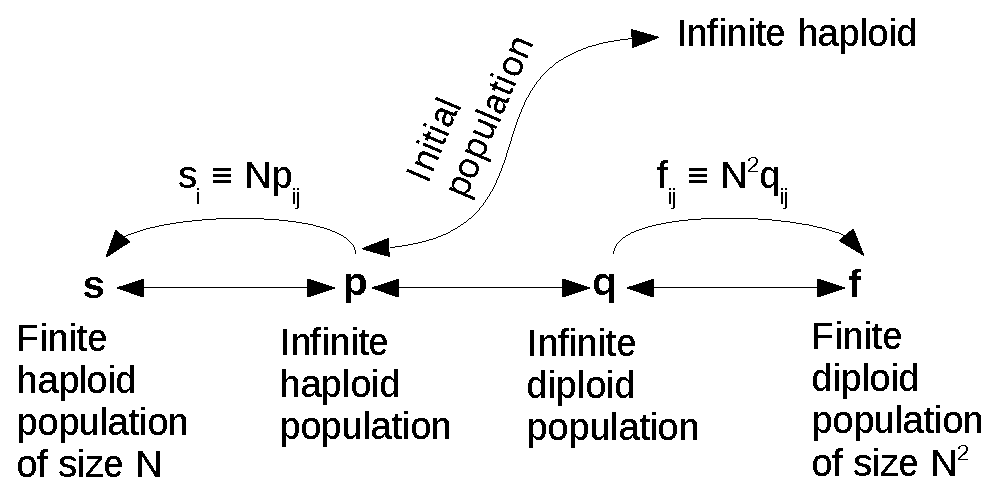
\includegraphics{figures/eps/initialpop.eps}}\hspace{5pt}
\caption{\textbf{Initial population computation:} }
\label{initalpop}
\end{center}
\end{figure}

Let finite haploid population $s^n$, finite diploid population $f^n$, infinite haploid population $p^n$ and infinite haploid population $q^n$ be considered with initial population $s^0$, $f^0$,
$p^0$, $q^0$ respectively. To investigate oscillating behavior of infinite population evolutionary limits and finite population, same initial population is desired. 

For a genome length $\ell$, let $x = 2^\ell$ be number of possible strings in finite haploid population array $t$ of population size $N$. Possible strings $t_i$ are ${0, 1,.., x-1}$ where $i = 0, 1,.., N-1$. An arbitrary vector $r$ of size $x$ was considered where
\[
r_i = U01(); {i = 0, 1,.., x-1}
\]
and U01() is random number between 0 and 1.
Let $t$ represent finite haploid population strings array.
\[
t_j = randp(r) ; {j = 0,.., N-1}
\]
where $t_j$ is $j^{th}$ population member and $randp(r)$ returns random index $i$ in array $r$ with probability $r_i$.

Let $c_i$ represent count of haploid member $i$ in population $t$ given by
\[
c_i = \sum \limits_{j=0}^{N-1} [t_j = i]  \nudge; \nudge {i = 0,.., x-1}  and  [..]  is  Iverson bracket
\]

Then infinite population vector $p$ is calculated as
\[
p_i = \frac{c_i}{ \sum \limits_{k=0}^{x-1} c_k }
\]
where $i = 0,.., x-1$ and $\sum \limits_{k=0}^{x-1} c_k = N$.

This $p$ is randomly generated initial infinite haploid population vector ($p^0$) which corresponds to diploid infinite population vector $q$ 
and finite population vectors $s$ and $f$.

Finite haploid population members $t_j$s are generated again to match finite haploid population $s^0$ with infinite haploid population $p^0$.
\[
c_i = N \cdot p_i 
\]
\[
\sum \limits_{j=0}^{N-1} [t_j = i] = c_i  \nudge; \nudge {i = 0,.., x-1} 
\]

Initial infinite diploid population $q_0$ is calculated corresponding to initial haploid population $p^0$ as
\[
q_{i,j} = p_i \cdot p_j  \nudge; \nudge {i = 0,..,x-1; j = 0,..,x-1}.
\]

Let $v$ represent finite diploid population member array of size $N^2$ and $d_{i,j}$ represent count of diploid member $\langle i,j \rangle$ in $v$. Then $v$ can be filled with population member to match initial population vector $p$ generating diploid members such that
\begin{eqnarray*}
d_{i,j} = N \cdot p_i \cdot N \cdot p_j 
\sum \limits_{k=0}^{N^2-1} [ v_k = \langle i,j \rangle ] = d_{i,j}
\end{eqnarray*}

Finite diploid population vector $f$ can be obtained from finite diploid population member array $v$  using
\[
f_{i,j} = \frac{d_{i,j}}{\sum \limits_{k=0}^{x-1} \sum \limits_{h=0}^{x-1} d_{k,h}}
\]
where $i = 0,.., x-1$, $h = 0,.., x-1$ and $\sum \limits_{k=0}^{x-1} \sum \limits_{h=0}^{x-1} d_{k,h} = N^2$.

This initial infinite haploid population vector $p^0$ corresponds to initial infinite diploid population vector $q^0$, initial finite 
haploid population vector with population size $N$ and initial finite diploid population vector $N^2$ with population size $N^2$.

\section{Oscillation}
\label{Oscillation}

Equations (\ref{lt1}) and (\ref{lt2}) were implemented with crossover distribution $\chi$ and mutation distribution $\mu$ satisfying 
condition (\ref{OscCond}) to investigate oscillating behavior of predicted infinite population evolutionary limits $p^{\ast} and q^{\ast}$ 
and finite population under no selective pressure.

Infinite haploid population evolutionary limits $p_h^{\ast}$ and $q_h^{\ast}$ were computed using equations (\ref{lt1}) and (\ref{lt2}). 
Infinite diploid population evolutionary limits $p_d^{\ast}$ and $q_d^{\ast}$ as
\begin{eqnarray*}
{p_d^{\ast}}_{\langle \gamma_0, \gamma_1 \rangle} & = & {p_h^{\ast}}_{\gamma_0} {p_h^{\ast}}_{\gamma_1} \\
{q_d^{\ast}}_{\langle \gamma_0, \gamma_1 \rangle} & = & {q_h^{\ast}}_{\gamma_0} {q_h^{\ast}}_{\gamma_1}
\end{eqnarray*}
where $\gamma = \langle \gamma_0, \gamma_1 \rangle$ is diploid genome.

For a genome length $\ell$, same initial population (calculated as described in (\ref{InitPopOsc})) was used for infinite population and all 
sizes of finite population conisdered.
Genome lengths $\ell = {2, 4, 6, 8, 10, 12, 14}$ were used. Minimum population size of $N_0 = 64$ was considered for finite haploid case and 
different population sizes $N = \{1N_0, 2N_0,.., 20N_0\}$ were considered. Finite diploid population was set as squared size of haploid 
population $N^2$.
The distances of $p^n$ and $s^n$ to haploid evolutionary limits $p_h^{\ast}$ and $q_h^{\ast}$ were plotted and the distances of $q^n$ and 
$f^n$ to diploid evolutionary limits $p_d^{\ast}$ and $q_d^{\ast}$ were plotted.


\section{Violation}
The results showed when $\chi$ and $\mu$ distributions satisfies (\ref{OscCond}), oscillation occurs in both infinite and finite population. 
Error $\epsilon$ was introduced to $\mu$ distribution and $\chi$ distribution such that (\ref{OscCond}) did not satisfy anymore and 
$x_g \neq −1$ for all $g$ ($x_g$ and $g$ defined in \ref{Limits}) so that $p^\ast = q^\ast$.

$\mu$ distribution was treated with $\epsilon$ such that
\[
\mu_i = (1-\epsilon) \mu_i ; i = \{0, 1, 2,.., 2^{\ell}-1\}.
\]
So that sum of $\mu$ distribution becomes, 
\[
1-\epsilon = \sum \limits_{i=0}^{2^{\ell}-1} \mu_i
\]
Then set
\[
\mu_0 = \epsilon
\]

$\chi$ distribution was treated with $\epsilon$ such that
\[
\chi_i = (1-\epsilon) \chi ; i = \{1, 2,.., 2^{\ell}-1\} 
\]
So that 
\[
\chi_k + \chi_{k+ g} = 1-\epsilon ; g is defined in \ref{Limits}
\]

Then $j$ is chosen where $\chi_j = 0$ and set $chi_j = \epsilon$. \newline

Simulations were run again with the violations in (\ref{OscCond}) implemented. Genome lengths $\ell = {2, 4, 6, 8, 10, 12, 14}$ were considered. 
Different finite hapliod population sizes $N = \{1N_0, 2N_0,.., 20N_0\}$ were considered. Finite diploid population was set as 
squared size of haploid population $N^2$.\newline
Let ${p1}_h^{\ast}$ and ${q1}_h1^{\ast}$ be haploid evolutionary limits with violation and ${p1}_d^{\ast}$ and ${q1}_d^{\ast}$ be diploid 
evolutionary limits with violation. The distances of ${p}^n$ and $s^n$ to ${p1}_h^{\ast}$ and ${q1}_h1^{\ast}$ were plotted and the distances of 
$q^n$ and $f^n$ to ${p1}_d^{\ast}$ and ${q1}_d^{\ast}$ were plotted.








 
